%----------------------------------------------------------------------------
\chapter{Graph neural network}\label{sect:GraphNetwork}
%----------------------------------------------------------------------------

\section{Neural Networks}
Artificial neural networks are used for various machine learning and deep learning purposes. In this section I will introduce the basic concepts of artificial neural networks used for supervised learning. Supervised learning is the process of neural network training with a given set of inputs and desired outputs and the goal is to train that system to predict the target outputs with the least error possible.

Most of the contents of this section is from the paper written by \'Ad\'am Kov\'acs and I for the Scientific Students' Associations conference in 2018 \cite{SemParse}.

\subsection{Perceptron}
The perceptron is the building block of the most basic neural networks. It functions as follows: The \(x\) input vector is element-wise multiplied by the \(w\) weight vector and is summed with the \(b\) bias parameter.
\[y = b + \sum_{i=1}^{n} x_i w_i\]

\begin{figure}[!ht]
	\centering
	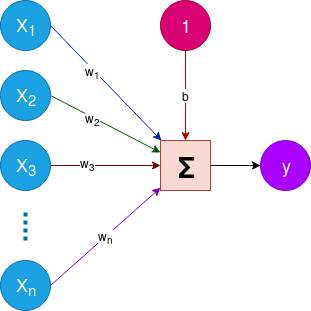
\includegraphics[width=75mm, keepaspectratio]{figures/perceptron.png}
	\caption{A perceptron.}
	\label{fig:perceptron}
\end{figure}

\subsection{Feed forward neural network}

The feed forward or dense neural network is built from perceptrons organized in layers, each layer fully connected to the next layer. The connections each have a weight parameter assigned to them. The nodes are perceptrons with only one slight difference, their output is not necessarily linear.

So called activation functions are used after the summation to bring non-linearity to the model. Such functions are for example the sigmoid, hyperbolic tangent, ReLU functions.

\[\sigma(x) = \frac{1}{1 + e^{-x}}\]
\[tanh(x) = \frac{e^x - e^{-x}}{e^x + e^{-x}}\]
\[relu(x) = \begin{cases}
	x, & \text{if } x > 0\\
	0, & \text{otherwise}
\end{cases}\]

So the result of one neuron in a layer is calculated as follows:

\[\hat{y} = activationFunction(\sum_{i=1}^{m}(x_i * w_i + b))\]

\begin{figure}[!ht]
	\centering
	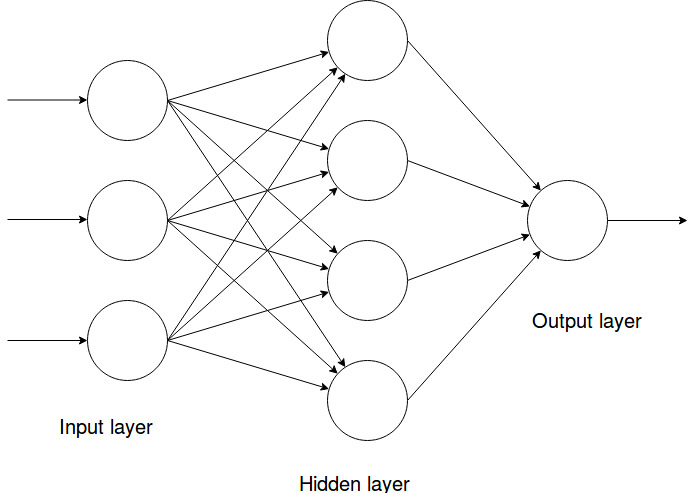
\includegraphics[width=125mm, keepaspectratio]{figures/feed_forward_neural_network.jpg}
	\caption{A feed forward neural network.}
	\label{fig:feed_forward}
\end{figure}

The weight and bias parameters are modified during a process called backpropagation which utilizes the chain rule to propagate the gradient of the loss backwards. The weights and the bias are updated with their difference from the gradient multiplied by a learning rate.

The loss is the difference function between the calculated value and the expected outcome. We don't just calculate the numeric difference in this case, but in case of classification we use the cross entropy function.

\[L = - \sum_{i=1}^{n} y_i \ln(\hat{y_i})\]

The equation above can be used in a multiclass system, where \(n\) is the number of classes and \(\hat{y}\) is the calculated output, while \(y\) is the expected output.

The parameter update happens as follows:

\[\Delta_x L = \sum_{k} \frac{\delta L}{\delta w^k}\frac{\delta w^k}{\delta x}\]

\[w \leftarrow w - \eta \Delta_x L\]

Where \(\eta\) is the learning rate.

The learning rate parameter can also change during the training process. This is called optimization. The main goal of it is to overcome the problems with setting the learning rate (too high can cause us to jump over any good solution, too low results in very slow learning and settling in a local minimum).

One such optimization method is called Adam. It is a cross between two other methods: Adaptive learning rate and Momentum. I used it for the training the models described in the next chapter. The basic idea is slowly degrading the learning rate, based on the previous gradient.

\subsection{Embedding layers}

The function of embedding layers is to turn values to fixed length vectors. They are used mostly in natural language processing to work as word2vec translation. Word2vec is the mechanism to translate a word into vector space.\cite{Word2Vec}

Word embeddings are used in basically all state-of-the art systems related to
natural language processing applications. Mikolov\cite{Mikolov:2013x} showed that word embeddings can be applied for vector operations, like addition or subtraction, and these operations often result in meaningful representation. If we have example words "King", "Man", "Woman", then the vector("King") - vector("Man") + vector("Woman") will most likely result in vector that is close to vector("Queen") in the embedding space. See Figure~\ref{fig:worvec}.

\begin{figure}[!ht]
	\centering
	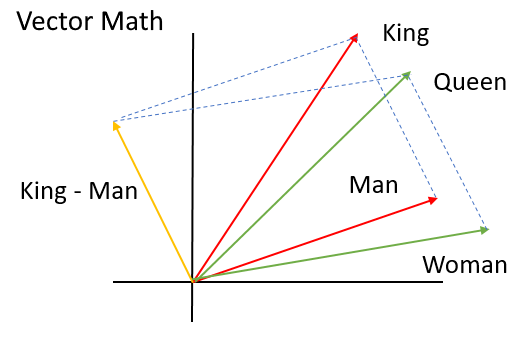
\includegraphics[scale=0.75, keepaspectratio]{figures/vecs.png}
	\caption{An word vector operations.}
	\label{fig:worvec}
\end{figure}

When using embedding layers we want to find vectors for each word so that it can model the word's meaning. We achieve this by looking at the context, the word usually appears in. If two words like \textit{apple} and \textit{orange} usually appear in the same context, than the vectors assigned to these words should have low cosine distance between them.

If you are building an NLP model, the embedding layer should be in the first layer, since its purpose is to make the transition from word to vector, and the word in this case is the input.

\begin{figure}[!ht]
	\centering
	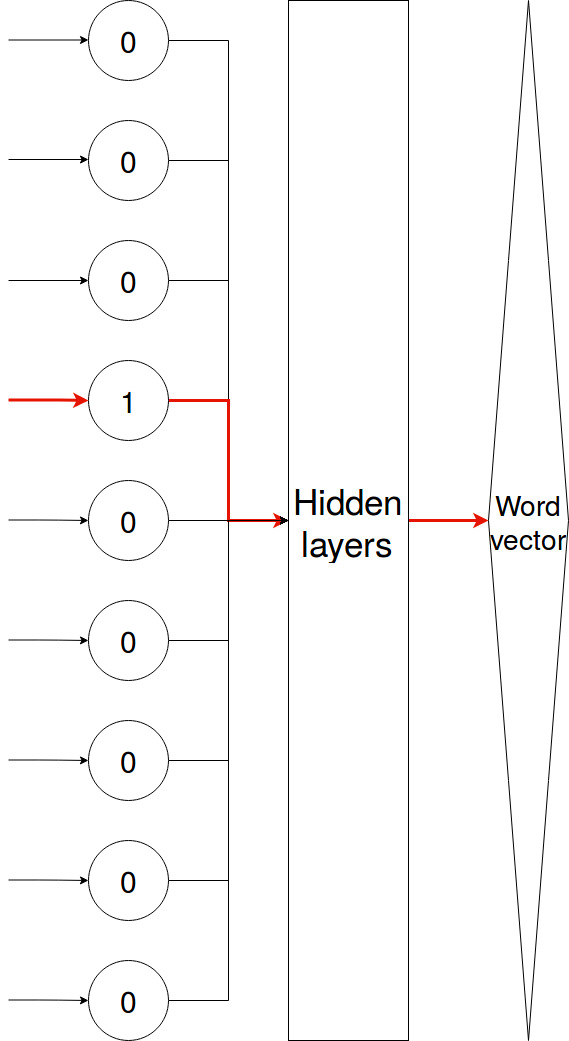
\includegraphics[scale=0.25, keepaspectratio]{figures/embedding_layer.jpg}
	\caption{An embedding layer.}
	\label{fig:embedding_layer}
\end{figure}

The input dimension of this layer is the size of the vocabulary and the output dimension is the size of the dense vector. Usually the vocabulary size greatly exceeds the embedding dimension since the output vectors size is fixed and can range from 300 to 1000, and the vocabulary - depending on the dataset - can be way higher than that. See at Figure~\ref{fig:embedding_layer}.

They work mostly like a lookup table that can be trained. A lot of the times we use pretrained models, like the GloVe embeddings\cite{GloVe} that have been trained on enormous datasets. We can also train them on our specific problem, or use the pretrained and our own embeddings simultaneously.

There has been a huge step forward on this field with the appearance of pre-trained embeddings built from language models. The first such embedding is ELMo \cite{ELMo} which is a deep-contextualized word representation capable to handle character level features as well as the context of a given word.

\subsection{Recurrent Neural Networks}

RNNs~\cite{RNN} can be used in supervised and also unsupervised learning. They are used when the data is sequential, like text, audio, etc.

\begin{figure}[!ht]
	\centering
	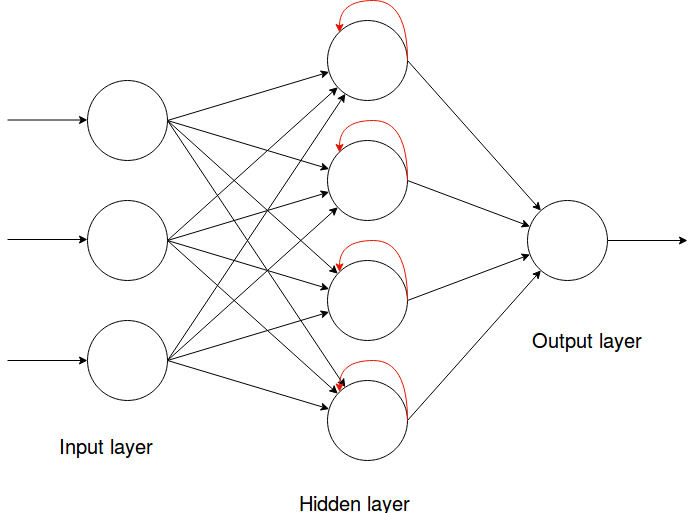
\includegraphics[width=125mm, keepaspectratio]{figures/recurrent_neural_network.jpg}
	\caption{A recurrent neural network.}
	\label{fig:recurrent_net}
\end{figure}

In a simple feed forward neural network, the information only moves in one direction: from the input layer to the output layer. On the other hand recurrent neural networks take into account their immediate past, the output of the network with the previous timestamp. This internal "memory" like functionality allows the network to remember what it had calculated before. This is illustrated at Figure~\ref{fig:recurrent_net}.

At every timestamp the network gets two sets of inputs: the actual input at the timestamp and the hidden state of the network for the previous input. In one iteration it calculates its output using the calculated hidden state in the timestamp. It all could be imagined like the same feed forward network being repeated after one other.

The hidden state mentioned above is the "memory" of the network that is calculated with the previous hidden state and the input.

\begin{figure}[!ht]
	\centering
	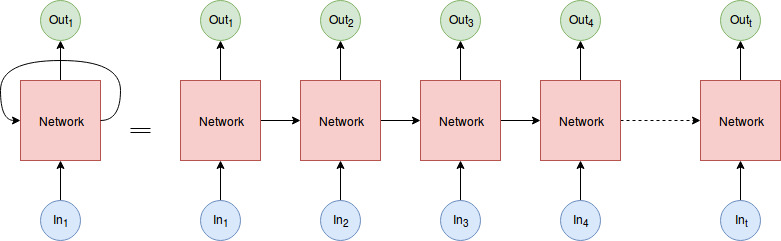
\includegraphics[width=150mm, keepaspectratio]{figures/unrolled.jpg}
	\caption{Unrolled recurrent neural network.}
	\label{fig:unrolled}
\end{figure}

The backpropagation is also slightly different in this case, it's called backpropagation through time, you need to "unroll" the network (see at Figure~\ref{fig:unrolled}), and use the backpropagation starting from the right timestamps. Each timestamp's backpropagation could be understood as backpropagation on a separate feed forward neural network.

The gradient vanishing or explosion can be a problem with this RNN.

There is a multitude of solutions for the exploding gradients, one of which is called gradient clipping. This technique is a very simple yet powerful way of dealing with exploding gradients. All it does is that it limits the size of the gradient, if its norm is higher than a set threshold.

\subsubsection{Long-Short Term Memory}
Long-short term memory networks\cite{LSTM} are the extension of the previously discussed recurrent neural network. The main difference is that it also has an internal long term memory. Usually these type of networks are more reluctant to have the exploding gradient problem.

Like the simple RNN, LSTMs also have hidden states, that are calculated slightly differently.
\\

\begin{minipage}{\textwidth}
	The LSTMs hidden states are calculated using three gates:
	\begin{itemize}
		\item \textbf{input gate}: determines whether to let new input in
		\item \textbf{forget gate}: determines whether to forget an input because it's not relevant anymore
		\item \textbf{output gate}: determines whether to let the input impact the output with the current timestamp
	\end{itemize}
\end{minipage}

These gates are analog and their values ranges from 0 to 1 with the sigmoid function. A simplified depiction can be seen at Figure~\ref{fig:lstm}.
\begin{figure}[!ht]
	\centering
	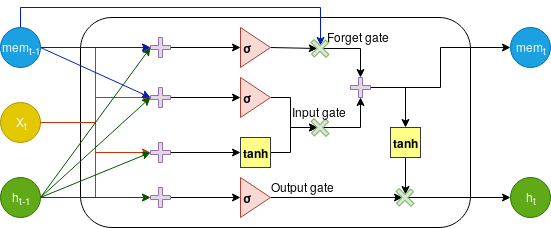
\includegraphics[width=125mm, keepaspectratio]{figures/lstm.png}
	\caption{A long-short term memory network's gates.}
	\label{fig:lstm}
\end{figure}

The sigmoid function allows this structure to be able to learn, meaning that we can use the backpropagation through time method described above.

Long-short term memory networks are used in natural language processing, but also in generative networks, like video or image description generation, text generation and so on.

\subsection{Attention}
The Attention mechanism was first described by Dzmitry Bahdanau in 2015 \cite{Bahdanau:2015} and was used for machine translation. Since then it became a widely used tool in natural language processing. The idea behind this mechanism is that when the neural network predicts the output, it only uses parts of the given input instead of the full input. That is where the most relevant information is concentrated and this mechanism only pays \textit{attention} to these parts and the network has to learn what to pay attention to.

Usually in the "sequence-to-sequence" tasks like machine translation there are two main parts of the model an encoder and a decoder. The encoder and the decoder are usually some type of RNN, mostly LSTM. The encoder is responsible for creating a so called context-vector from the input sequence. This context-vector has a fixed length and it serves as the representation of the sequence inside the model. The decoder then decodes this context-vector to a sequence again, in the case of the machine translation this sequence is in a different language. A depiction can be seen at Figure~\ref{fig:seq_to_seq}.
\begin{figure}[!ht]
	\centering
	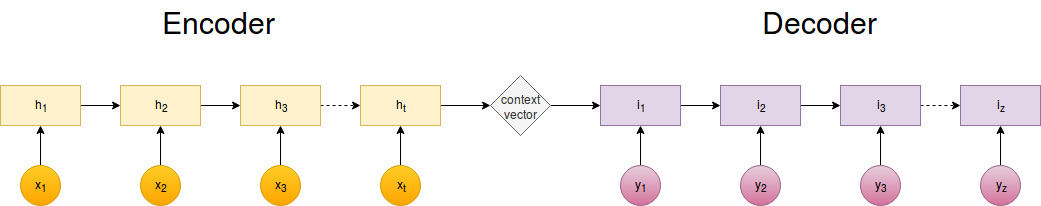
\includegraphics[width=150mm, keepaspectratio]{figures/seq_to_seq.jpg}
	\caption{A sequence-to-sequence model with encoder and decoder.}
	\label{fig:seq_to_seq}
\end{figure}

The attention mechanism was used in the decoder part of this model, the encoder functions the same way. The paper explicitly stated that this attention mechanism relieves the encoder from having to encode every sequence to a fixed length context vector. In this case we have a context vector for every word of the expected output. These context-vectors are the weighted sums of the encoder's states (\textit{annotations}).
\[c_i = \sum_{j=1}^{t} \alpha_ij h_j\]
Where \(\alpha\) parameter is calculated like the following:
\[\alpha_ij = \frac{exp(e_{ij})}{\sum_{k=1}^{t} e_{ik}} \]
and \(e_{ij}\) is its energy
\[e_{ij} = a(s_{i-i}, h_j)\]

\begin{figure}[!ht]
	\centering
	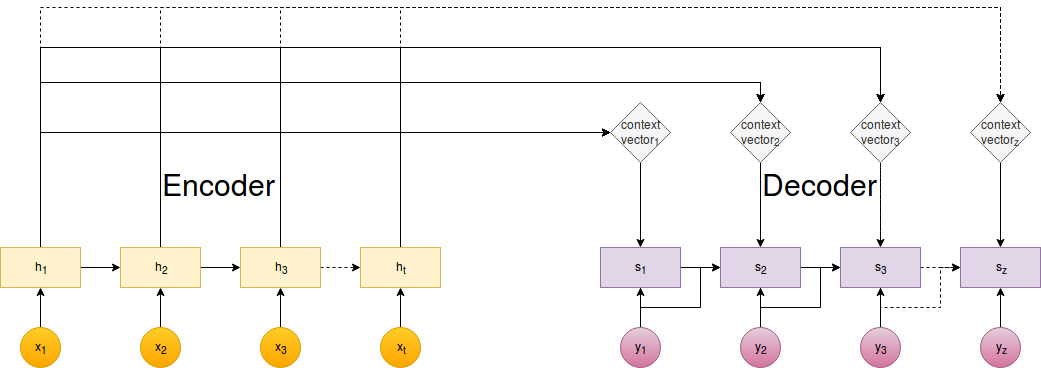
\includegraphics[width=150mm, keepaspectratio]{figures/attention.jpg}
	\caption{A sequence-to-sequence model with encoder-decoder and attention.}
	\label{fig:attention}
\end{figure}

This is an \textit{alignment model} that scores how well the input around \textit{j} and the output around \textit{i} match. This \textit{alignment model} is a feed forward neural network that is trained simultaneously with the other components of the system.
The decoder uses the previous state's output and its assigned context-vector when calculating its own target.
\[s_i = f(s_{i-1}, y_{i-1}, c_i)\]
The attention based model is at Figure~\ref{fig:attention}.


\section{The graph\_nets library}
As I mentioned in the previous chapter graph neural networks are used for graph transformation. Recently an article has been published about the types and possible uses of graph neural networks\cite{SurveyGNN}.  Graph neural networks are used on the field of physics\cite{PhysicsGNN}, computer vision\cite{CVGNN} and also NLP\cite{NLPGNN} but they are still not common.\footnote{\url{https://github.com/thunlp/GNNPapers}}

My main source for understanding the mechanisms of the graph\_nets library was the article titled \textit{Relational inductive biases, deep learning, and graph networks}\cite{GraphNet} and the \href{https://github.com/deepmind/graph_nets/tree/master/graph_nets/demos}{demos} available on GitHub.
The article explains the different approaches of graph transformation learning, most importantly the graph independent model and the graph dependent models.

The most notable difference between the two is the fact that while the graph dependent structure uses the data of the nodes and the edges simultaneously, the graph independent model does train the nodes and edges separately from each other.

Both models can be used under different circumstances, but the can also be used together in training processes.

\subsection{Graph Network block}

The graph\_nets library contains three different block type: EdgeBlock, NodeBlock and GlobalBlock. Each responsible for the propagation of the corresponding tensor through the right function. So we can construct different models for edges, nodes and global parameters.

\textbox{
	\textbf{Definitions from the code}

	The \textit{NodeBlock} updates the features of each node in batch of graphs based on
	the previous node features, the aggregated features of the
	adjacent edges, and the global features of the corresponding graph.
	
	The \textit{EdgeBlock} updates the features of each edge in a batch of graphs based on the previous edge features, the features of the adjacent nodes,
	and the global features of the corresponding graph.
	
	The \textit{GlobalBlock} updates the global features of each graph in a batch based on the previous global features, the aggregated features of the
	edges of the graph, and the aggregated features of the nodes of the graph.
}{}

On top of using these graph structure dependent building blocks the GraphNetwork model (or Graph dependent model for the sake of clarity) it utilizes the updated edge features to calculate the node features and these results are used to update the global features.

\subsection{Graph Independent block}
As the name suggests, in this block every aspect of the graph is independent from another, the defined update functions only take into account their input tensor which can be the node tensor, the edge tensor or the global tensor.

\subsection{Self Attention block}
The graph\_nets library contains a multi-head self attention module which is mostly based on the article titled Attention Is All You Need~\cite{Multihead} which introduced Multi-head attentions.

This mechanism updates the node features based on the node values, node keys and node queries taking into account the structure of the graph.